\section{Poświęcenie palm i procesja}

\begin{itemize}
	\item w tej części \dd~ całuje \ii~ standardowo jak podczas mszy,
	\item podczas ubierania celebransa asystuje \cc, kolejno diakona \aa1 oraz
	      subdiakona \aa2,
	\item ustawiamy się w szyku procesyjnym. Lewci przez cały czas procesji i
	      poświęcenia ,jeżeli jest to możliwe, trzymają kapę. Wychodzimy przez
	      główne wyjście na zewnątrz. Przy przechodzeniu przez oś ołtarza
	      polowego, przyklękają wszyscy oprócz: \ding{63}, \aa1, \aa2 oraz \ii,
	\item schola śpiewa podczas procesji \textit{Hosanna filio David} na
	      przemian z Psalmem 117 \footnote{Zob. \textit{Liber Usualis} z 1961 :
		      Ritus servandus in celebratione Missae in Cantu ad 1.},
	\item po dojściu na miejsce święcenia palm, \cc~ odbiera nakrycia głowy,
	      następuje  oddanie referencji ołtarzowi przez lewitów oraz \ii~
	      (lewici przyklękają, \ii~ głęboko się skłania), \ii~ całuje ołtarz
	      następnie ustawiamy się w sposób przedstawiony na Rys. 1,
\end{itemize}

\bigskip

\begin{figure}[h]
	\centering
	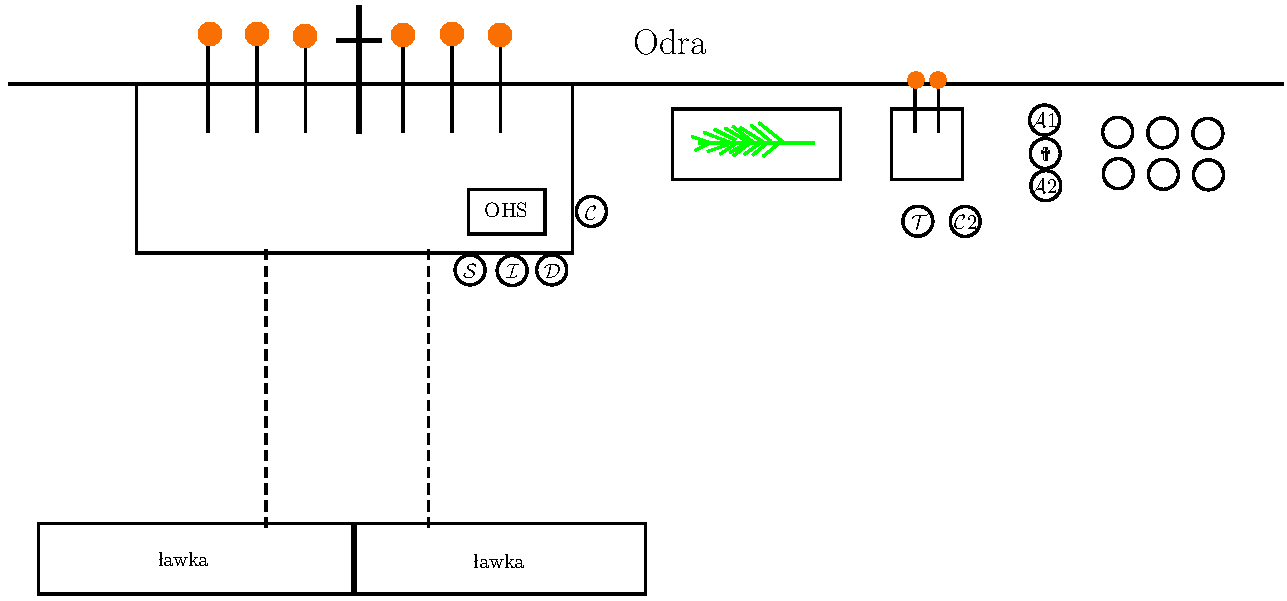
\includegraphics[width=\linewidth]{Palmowa/PalmyNadOdra.pdf}
	\caption{Ustawienie po przyjściu do ołtarza}
\end{figure}

\bigskip

\begin{itemize}
	\item \ii~ cicho odczytuje antyfonę \textit{Hosanna filio David}, tak jak
	      podczas Mszy, a następnie śpiewa \textit{Dominus vobiscum}, zwrócony w
	      kierunku księgi,
	\item po \textit{Amen} następuje zasypanie,
	\item \aa1 podaje wodę \cc~ a ten podaje ją \dd,
	\item następuje pokropienie, \aa1 odbiera wodę od \dd,
	\item następuję okadzenie,
	\item palmę dla \ii~ \dd~ kładzie na ołtarzu,
	\item następuje rozdawanie palm (\cc2 podaje palmy, \cc1 zawiaduje ruchem),
	      odbieranie palm od \ii~ z pocałunkiem, asysta ustawia się dwójkami jak
	      do komunii w kolejności: lewici, klerycy, ministranci, lud,
	\item po rozdaniu palm \ii~ myje ręce, pomagają mu w tym \aa,
	\item następuje odśpiewanie ewangelii, nie przenosi się mszału,
	\item do ewangelii ustawiamy się jak podczas mszy, gdy już dojdziemy na
	      miejsce jak na Rys 2,

	      \begin{figure}[h!]
		      \centering
		      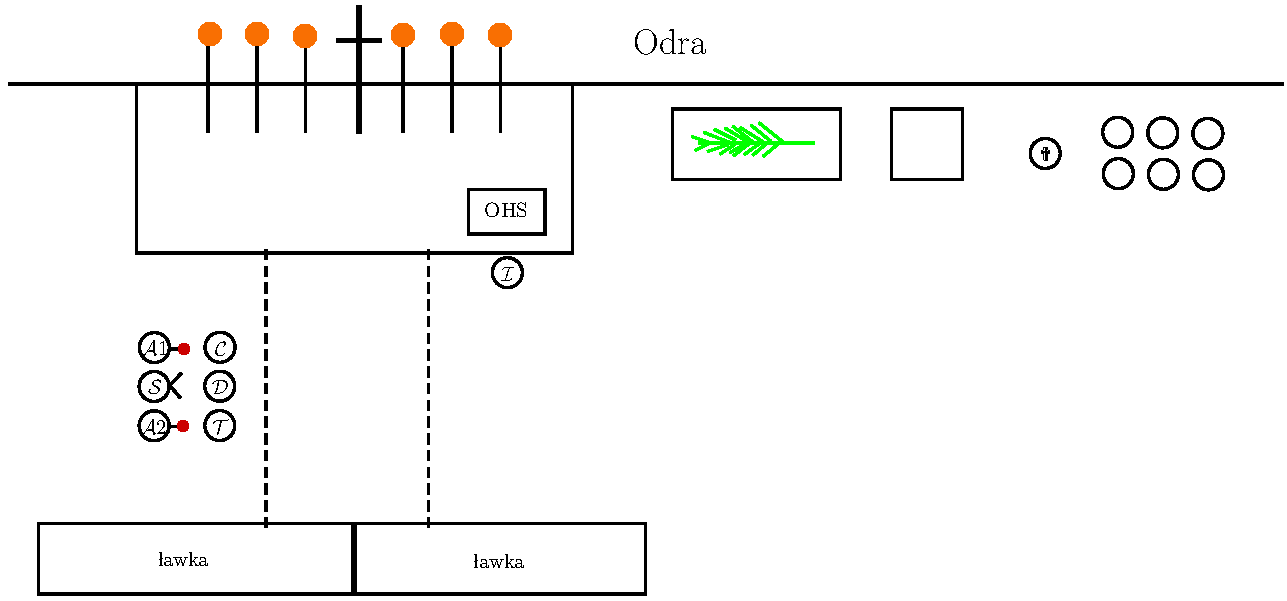
\includegraphics[width=\linewidth]{Palmowa/PalmyNadOdra2.pdf}
		      \caption{Ustawienie podczas Ewangelii}
	      \end{figure}

	\item po odśpiewaniu ewangelii \ii~ całuje ewangeliarz oraz jest okadzany
	      przez \dd,
	\item kantorzy ($A$) oraz mikrofoniarz udają się najkrótszą możliwą drogą do
	      pierwszych drzwi kościoła. Przymykają je lekko, ale obserwują, czy
	      procesja już się zbliża. Dwóch lub jeden Kantor ($B$) pozostaje w
	      procesji z ministrantami,
	\item po powrocie do pozycji z Rys 1 następuje zasypanie,
	\item lewici stają w rzędzie za	\ii,
	\item \dd~ staje obok rzędu i śpiewa \textit{Procedeamus in pace},
	\item Kantor ($B$) oraz mikrofon wraz z ludem śpiewa \textit{In nomine
		      Christi. Amen}, a następnie rozpocznie jedno z poniższych:

	      \begin{itemize}
		      \item śpiew jednej z antyfon procesyjnych z \textit{Liber
			            Usualis},
		      \item \textit{Christus vincit},
		      \item pieśń po polsku do Chrystusa Króla;
	      \end{itemize}

	\item po oddaniu rewerencji ołtarzowi \cc~ oddaje nakrycia głowy,
	\item ustawiamy się w szyku procesyjnym, Kantor/Kantorzy ($B$) zajmują w
	      procesji miejsce zaraz za \ding{63},
	\item udajemy się w kierunku bocznych drzwi po schodach za pomnikiem biskupa
	      Kominka,
	\item kantorzy A wewnątrz kościoła obserwują delikatnie, czy procesja
	      nadchodzi,
	\item kiedy procesja dochodzi do drzwi Kościoła, \ss~ z \aa~ stają przodem
	      do drzwi, a ministranci rozchodzą się na boki tworząc szpaler tak aby
	      \ii~ znajdował się nieopodal \ding{63}, jak na Rys 3,

	      \bigskip

	      \begin{figure}[h]
		      \centering
		      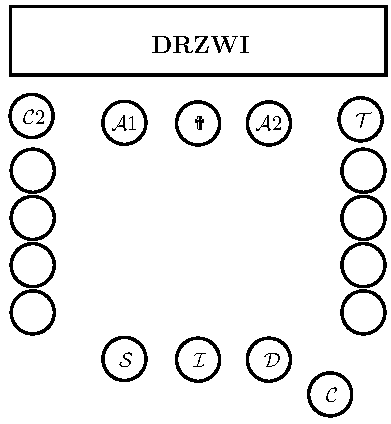
\includegraphics[width=0.26\linewidth]{Palmowa/PalmyNadOdra3.pdf}
		      \caption{Procesja przy drzwiach kościoła}
	      \end{figure}

	\item kantorzy ($A$) (w środku) stojąc zwróceni w kierunku drzwi śpiewają:
	      \textit{Gloria Laus et honor} etc.,
	\item kantorzy ($B$), ministranci i wierni powtarzają werset: \textit{Gloria
		      Laus},
	\item kantorzy ($A$) śpiewają poszczególne zwrotki hymnu, po każdej zwrotce
	      Kantorzy ($B$) + reszta odśpiewują refren: \textit{Gloria, Laus},
	\item po piątej zwrotce i refrenie \ding{63} głośno i widocznie uderza nóżką
	      krzyża procesyjnego w drzwi, a Kantorzy ($A$) i \cc2 szeroko otwierają
	      drzwi,
	\item \cc2 wprowadza \ding{63} i resztę procesji do wnętrza kościoła. W tym
	      czasie Kantorzy ($A$) i Kantorzy ($B$) łączą się w jedną grupę i jak
	      najszybciej zaczynają śpiew: \textit{Ingrediente Domino}, podany w
	      \textit{Liber Usualis};
	\item \dd~, \ss~, \ii~ oraz \cc~ po przyklęknięciu na środku udają się
	      bezpośrednio do księgi po stronie epistoły, reszta asysty i chór
	      przyklękają po kolei na środku. Wszyscy zajmują swoje miejsca i
	      odkładają palmy. \aa~ odkładają świece a \ding{63} krzyż
	\item modlitwa na zakończenie procesji od Mszału ustawionego przy ołtarzu po
	      stronie Epistoły, lewici trzymają brzegi kapy (jak przy poświęceniu),
	\item po skończonej oracji, \ii~ i \dd~ oraz \ss~ podchodzą do sedilli i
	      przebierają się. Przebieranie przebiega w następującej kolejności:

	      \begin{itemize}
		      \item \cc~ zabiera kapę przekazuje zakrystianom,
		      \item lewici ściągają dalmatyki z pomocą \aa1 oraz \aa2 i \cc,
		      \item lewici ubierają w ornat \ii, zakrystianie zabierają w tym
		            czasie dalmatyki i manipularze czerwone
		      \item \aa1 zakłada tunicelę \ss, \aa2 dalmatykę \dd,
		      \item \cc~ sprawdza czy \dd~ i \ss~ mają swoje szaty
	      \end{itemize}

\end{itemize}

\enlargethispage{20pt}

%	\section{Poświęcenie palm}
%
%	    \begin{itemize}
%	      \item wszyscy procesyjnie udają się do ołtarza w kolejności:
%
%	        \begin{enumerate}\centering
%	         \item[] $\mathcal{T}$~~~$\mathcal{C}2$
%	         \item[] $\mathcal{A}1$~~~\ding{63}~~~$\mathcal{A}2$ 
%	         \item[] reszta chóru parami
%	         \item[] $\mathcal{C}1$
%	         \item[] $\mathcal{S}$~~~$\mathcal{I}$~~~$\mathcal{D}$
%	        \end{enumerate}
%
%	        \item po przklęknięciu wszyscy udają się na swoje miejsca -- chór \textbf{stoi}
%	        \item \sout{$\mathcal{A}1$ i $\mathcal{A}2$ zanoszą stolik z palmami na środek prezbiterium} stolik jest już wyniesiony
%	        \item $\mathcal{I}$ z $\mathcal{D}$ i $\mathcal{S}$ udają się do stolika z palmami (twarzą do ludzi)
%	        \item $\mathcal{T}$ i $\mathcal{C}2$ stają przy stoliku po stronie Ewangelii, a $\mathcal{C}1$ - Epistoły
%
%	        \begin{figure}[h]
%	          \centering
%	          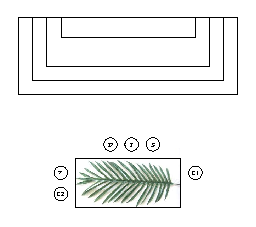
\includegraphics[scale=3]{Palmy.eps}
%	        \end{figure}
%
%	        \item następuje błogosławieństwo, pokropienie palm, zasypanie kadzidła i okadzenie palm \footnote{Małaczyński s. 59-60}
%	        \item $\mathcal{I}$ z $\mathcal{D}$ i $\mathcal{S}$ idą do ołtarza, a chór ustawia się parami tak, jak do Komunii
%
%	        %\newpage
%
%	        \item palmy odbierane są przez ministrantów parami w sposób następujący:
%	          \begin{enumerate}[leftmargin=1cm]
%	           \item przyklęknięcie na posadzce
%	           \item wejście po stopniach i uklęknięcie na ostatnim
%	           \item odebranie palmy \textbf{z pocałunkiem} w dłoń $\mathcal{I}$
%	           \item powstanie, przyklęknięcie w miejscu i udanie się w swoje miejsce
%	          \end{enumerate}
%	        \item $\mathcal{I}$ z $\mathcal{D}$ i $\mathcal{S}$ rozdają palmy ludowi -- chór \textbf{siada}
%	        \item $\mathcal{A}1$ i $\mathcal{A}2$ zabierają stół z palmami, gdy kończy się ich rozdawanie
%	        \item $\mathcal{A}1$ i $\mathcal{A}2$ asystują przy obmyciu rąk $\mathcal{I}$ (przy kredensji)
%	        \item $\mathcal{I}$ z $\mathcal{D}$ i $\mathcal{S}$ idą do ołtarza, a tam następuje zasypanie kadzidła
%
%	        \newpage
%
%	        \item formuje się procesja do Ewangelii (patrząc od ołtarza):
%	          \begin{enumerate}\centering
%	           \item[] (stopnie ołtarza)
%	           \item[] $\mathcal{S}$~~~$\mathcal{D}$
%	           \item[] $\mathcal{C}$1~~~$\mathcal{T}$
%	           \item[] $\mathcal{A}$2~~~$\mathcal{A}$1
%	          \end{enumerate}
%	        \item na znak ceremoniarza formacja klęka i udaje się w wyznaczone miejsce
%
%	        \begin{figure}[h]
%	          \centering
%	          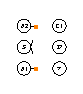
\includegraphics[scale=3]{Ewangelia.eps}
%	        \end{figure}
%
%	        {\color{Red} \item chór na czas Ewangelii wstaje i obraca się w twarzą do \underline{\textbf{\color{Red}Ewangeliarza}} (i w tamtym kierunku wykonuje wszystkie skłony przepisane)}
%	        \item po Ewangeli $\mathcal{S}$ i $\mathcal{C}1$ udają się do $\mathcal{I}$
%	        \item $\mathcal{A}$1 i $\mathcal{A}$2 idą na środek prezbiterium (przy balaskach) i tam czekają 
%	        \item $\mathcal{D}$ i $\mathcal{T}$ udają się do ołatarza, żeby zasypać kadzidło
%	      \end{itemize}
%
%	\section{Procesja z palmami}
%
%	    \begin{itemize}
%	     \item następuje zasypanie przy ołtarzu
%	     \item w międzyczasie formuje się procesja (kolejność taka sama, jak przy wejściu)
%	     \item podczas śpiewania \textit{Procedamus in pace} $\mathcal{I}$ ,$\mathcal{D}$ i $\mathcal{S}$ stoją jeden za drugim
%	     \item na znak $\mathcal{C}1$ ministranci klękają (oprócz $\mathcal{A}1$, $\mathcal{A}2$ i \ding{63}) i rusza prosceja prowadzona przez $\mathcal{C}2$ 
%	     \item po dojściu do stopni ołtarza, ministranci przyklękają parami i udają się na swoje miejsca, a chór stoi
%	     \item $\mathcal{C}2$ zanosi na ołtarz Mszał i stawia go po stronie Epistoły
%	     \item $\mathcal{I}$ z $\mathcal{D}$ i $\mathcal{S}$ przyklękają i udają się po skosie na stronę Epistoły (stają jeden za drugim)
%	     \item $\mathcal{I}$ śpiewa \textit{Dominus Vobiscum} bez odwracania się do ludu \footnote{Część współczesnych liturgistów zajmujących się klasycznym rytem zwraca uwagę na to, iż odmawianie modlitw versus populum, pomimo iż jest zawarte w rubrykach OHS, nie stanowi integralnej części rytu rzymskiego z 1962, lecz było wdrażanych jako część „uproszczonego rytu zreformowanego z 1965”. Zalecają zastosowanie w przypadku tych modlitw analogicznych rozwiązań z innych dni liturgicznych lub sprzed reformy Wielkiego Tygodnia. Poniższe rozwiązanie nawiązuje do oracji przy poświęceniu popiołu w Środę popielcową. Źródło: Cykl wykładów wygłoszonych przez ks. Svena Conrada FSSP w Wigratzbad w marcu 2015r.}
%	     \item po zaśpiewanej przez $\mathcal{I}$ oracji, udaje się on wraz z $\mathcal{D}$ i $\mathcal{S}$ krótką drogą do sedilii
%	     \item $\mathcal{I}$ z $\mathcal{D}$ i $\mathcal{S}$ zmieniają szaty, a pomagają im $\mathcal{A}1$, $\mathcal{A}2$, $\mathcal{C}1$
%	    \end{itemize}